%% MANUSCRIPT IN THE PROGRESS IN THIS DOC: PLEASE CONTRIBUTE THERE
%%https://docs.google.com/document/d/16clK-npH8XWA7p_llKXXWScyVuvJ1bjQ9kDyP1jmniw/edit?usp=sharing

\section{Introduction}\label{sec:introduction}
In recent years, Evolutionary Algorithms (EAs) have become increasingly prominent in training agents within complex environments, particularly in areas such as video game AI \cite{lucas2006evolutionary}.
Video games serve as ideal testing grounds for EA research, as they are characterized by dynamic, non-linear challenges and uncertainties, such as unpredictable enemies \cite{togelius2007computational, togelius2009super}.
These qualities need adaptive and robust solutions, often making traditional optimization methods less effective due to high-dimensional search spaces and non-stationary conditions \cite{yannakakis2018AIgames}.
By continuously interacting with the environment, agents trained via EAs can learn to navigate and adapt to the evolving challenges posed by these complex environments.

EAs are inspired by the principles of natural selection and biological evolution, where solutions evolve over successive generations using key genetic operators such as selection, crossover (also known as recombination), and mutation \cite{eiben2015bookEA}.
These operators are essential, as they allow for the exploration and exploitation of the solution space in search of optimal solutions.
Among them, crossover and mutation are the most critical as they both contribute to genetic diversity \cite{luke1997comparison}.

Crossover, which combines genetic material from parent solutions to generate offspring, is important for exchanging successful traits between individuals in the population.
This mechanism plays a critical role in promoting the discovery of high-performing solutions by allowing favourable traits to propagate and combine in new ways.
In contrast, mutation introduces random changes to individual solutions, ensuring diversity within the generation and preventing premature convergence by exploring previously unexplored areas of the search space.
While mutation is essential for maintaining variability within the population, it typically results in incremental changes (particularly in larger populations), often refining rather than drastically improving solutions (luke1997comparison).
Given the complexity of dynamic environments, crossover plays an important role in driving the rapid improvement of solutions, creating offspring that inherit the most effective traits from different individuals, and is therefore manipulated in this study.

\subsection{Research Question and Hypotheses}
The primary objective of this study is to evaluate the effects of these two crossover operators on the performance and convergence characteristics of an EA in training a specialist agent.
This leads us to the following research question:

\textit{What is the impact of BLEND and TWO-POINT crossover operators on the convergence and performance of an Evolutionary Algorithm in training a specialist agent in a video game playing python framework?}

\paragraph{Hypothesis 1}
The Blend Crossover operator will demonstrate a slower convergence rate compared to the Two-Point Crossover operator, due to its greater exploration of the solution space. In contrast, the Two-Point operator will demonstrate a faster convergence rate compared to Blend Crossover due to its more exploitative nature.
\paragraph{Hypothesis 2}
Specialist agents evolved using the Blend Crossover operator will achieve higher performance compared to those evolved using the Two-Point crossover operator.

We are developing, applying and comparing 2 EA (manipulating the crossover operators, one is blend crossover and the other one is two-point crossover) for the task of video game playing using a python framework called EvoMan to train a specialist agent (simulation mode “individual evolution”)

\subsection{The EvoMan Framework}
The EvoMan Framework is a Python-based platform designed for evaluating evolutionary algorithms in the context of game-playing agents, specifically inspired by the boss fights from Mega Man 2 de2016electronic).
EvoMan provides an environment where specialist agents, which are optimised to face specific enemies, can be trained.
It features eight distinct enemy bosses, each with unique behaviour that present different challenges in different environments to the player agent.
Both the player and the enemies start with 100 energy points, which are reduced each time they come into contact or are hit by the weapon \cite{2016evoman}.

\section{Method}
\subsection{Algorithm Description}
% 2 Point Crossover
\paragraph{2-Point crossover}
Two indices between 1 and $n-1$ are chosen randomly.
Both parents are split at the points specified by the indices.
The offspring is then created by glueing the split parts together, alternating between parents, which results in two children.
\begin{algorithm}
\caption{2-Point Crossover}\label{alg:2px}
\begin{algorithmic}

\Require $X^{(t)}, Y^{(t)}$
\State Choose two uniform random numbers $c_1, c_2 \in [1, n-1]$
\State $X^{(t+1)} \gets X^{(t)}[0:c_1] + Y^{(t)}[c_1:c_2] + X^{(t)}[c_2:n]$
\State $Y^{(t+1)} \gets Y^{(t)}[0:c_1] + X^{(t)}[c_1:c_2] + Y^{(t)}[c_2:n]$

\end{algorithmic}
\end{algorithm}

% Blend Crossover
\paragraph{Blend crossover}
For every pair of scalars $x_i^{(t)}, y_i^{(t)}$ from $X^{(t)}, Y^{(t)}$, respectively, a distance $d_i$ is calculated.
Using $d_i$ and the input parameter $\alpha$, an interval is constructed from which two real numbers are chosen randomly as the values for $x_i^{(t+1)}$ and $y_i^{(t+1)}$. \\
Blend crossover therefore introduces the additional hyperparameter $\alpha$ which scales the size of the interval the random values are chosen from.
\begin{algorithm}
\caption{Blend Crossover}\label{alg:blendx}
\begin{algorithmic}

\Require $X^{(t)}, Y^{(t)}$
\Ensure $\alpha \in \mathbb{R}_{\geq 0}$
\For{$i = 1, \dots, n$}
    \State $d_i \gets |x_i^{(t)} -  y_i^{(t)}|$
    \State Choose two uniform random real numbers
    \State $u_1, u_2 \in [\min(x_i^{(t)}, y_i^{(t)}) - \alpha d_i, \max(x_i^{(t)}, y_i^{(t)}) + \alpha d_i]$
    \State $x_i^{(t+1)} \gets u_1$
    \State $y_i^{(t+1)} \gets u_2$
\EndFor

\end{algorithmic}
\end{algorithm}

The two methods were chosen because they provide different advantages to the EAs. 
The 2-Point crossover creates offspring by combining different parts of the parents. 
This results in children that are only made up of discrete genes that are present in their parents, which also means being limited to the inside of the hypercube defined by the parents. 
2-Point crossover is therefore very exploitative.
Blend crossover, on the other hand, uses the parents genes only for determining the continuous range from which the new real values are drawn. 
This means that children are highly unlikely to share any genes with their parents 1 to 1 and also have the possibility to lie outside of the parents confines. 
Thus Blend crossover is highly explorative for a crossover operation.

\subsection{Experimental Setup}

\begin{table}[tbp]
    \begin{tabu}{|l|ll|}
    \hline
    Representation            & \multicolumn{2}{l|}{Real-valued vector}                  \\ \hline
    Recombination             & \multicolumn{1}{l|}{2-Point-Crossover} & Blend Crossover \\ \hline
    Recombination probability & \multicolumn{1}{l|}{70\%} & 70\%                         \\ \hline
    Mutation                  & \multicolumn{2}{l|}{Gaussian, $\mu$=0, $\sigma$=0.3}     \\ \hline
    Mutation probability      & \multicolumn{1}{l|}{10\%} & 5\%                          \\ \hline
    Parent selection          & \multicolumn{2}{l|}{Tournament selection, size=3}        \\ \tabucline[1.2pt]{-}
    Survival selection        & \multicolumn{2}{l|}{Replace all except best solution}    \\ \hline
    Population size           & \multicolumn{2}{l|}{100, variable}                       \\ \tabucline[1.2pt]{-}
    Number of offspring       & \multicolumn{2}{l|}{2}                                   \\ \hline
    Initialisation            & \multicolumn{2}{l|}{Random}                              \\ \hline
    Termination condition     & \multicolumn{2}{l|}{50 generations}                      \\ \hline
    \end{tabu}
    \caption{EA specification tableau.}
\end{table}

The experiment contains six training phases, three for each EA.
Both EA’s will be trained against the same three enemies to assess their performance individually on each enemy.
To optimize performance, the hyperparameters of both EAs are tuned by manual adjustments based on their prior performance.
Apart from the standard hyperparameters, the ones specific to our EA instances are the standard deviation and mean for the Gaussian mutation, the tournament size for the tournament selection and alpha for blend crossover.

An individual training phase consists of ten independent runs, each lasting fifty generations.
In every run one hundred initial individuals are evolved by the EA in order to maximize their fitness.
Over the ten runs the maximum fitness, average fitness and their standard deviation are recorded and the best solution is saved.
This yields two solutions for each of the three chosen enemies.

The results are represented in three figures, one for each enemy, showing the performance of both EA’s.

The two best solutions per enemy are tested against the enemy it has been trained on.
The testing is done by running the solution against the enemy five times and plotting the individual gain in a box plot.
[FIXME: is individual gain explained somewhere?]

To avoid over-fitting, randomini in the Evoman framework is turned on.
Randomini ensures the enemy is starting from a different place every time.
Because of the different starting positions, the EA has to use the enemies’ locational values to beat it.
Therefore, the testing will also be more accurate.

For the experiment, an enemy is needed to adjust the hyper parameters on.
For this task enemy 8 is chosen for several key reasons. First, enemies 1 and 8 jump, which adds complexity in tracking the enemy for the controller.
Training against a jumping enemy is expected to enhance the controller’s ability to handle more unpredictable movements.
This complexity can help to make sure the controller is evolving properly and is not getting stuck on local maxima.
Additionally, enemy 1 is the only enemy that fights on a battlefield with height differences.
By using a flat terrain, the environmental factors that could influence the controller’s behaviour are minimised thus giving a better representation of how the EA is performing.
Two more enemies are needed to test the EAs on. A relatively simple and a complex enemy is chosen for this.
The less complex enemy is enemy number 2.
This is a simpler version of enemy 8.
The complex enemy will be enemy 7.
This enemy fights in an underwater world with unlimited jumping and spikes on the ceiling.
\section{Results}

\subsection{Hypothesis 1}
The results confirm the prediction that the Blend Crossover operator demonstrates a slower convergence rate compared to the Two-Point Crossover operator across all enemies, which is shown as it crosses the convergence threshold faster.
The convergence threshold was set at 85\% of the maximum fitness value, at the fitness score of 80, which is where the fitness curve tends to flatten.

For Enemy 2, the EA using Two-Point Crossover crossed the threshold in generation 12, whereas the EA using Blend Crossover crossed the threshold in generation 19.
For enemy 7, the Two-Point Crossover crossed the threshold in generation 44, whereas Blend Crossover did not cross the threshold.
For Enemy 8, the Two-Point Crossover crossed the threshold twice, in generations 23 and 41, whereas Blend Crossover did not cross the threshold.
Additionally, the Blend Crossover showed a larger standard deviation across all enemies compared to the Two-Point Crossover.

\begin{figure}[htbp]
    \centering
    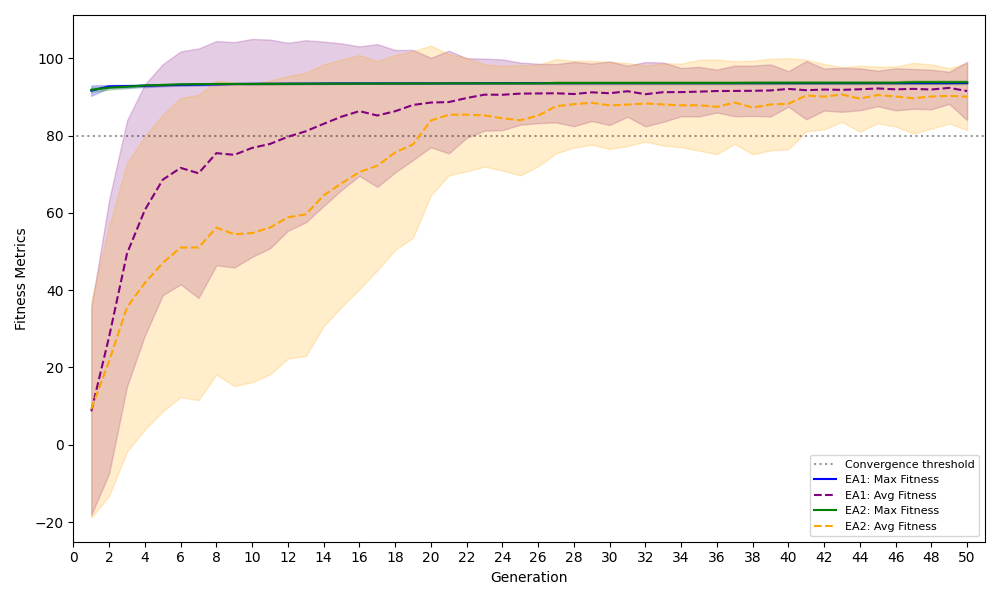
\includegraphics[width=\linewidth]{../../plots/enemy2}
    \caption{}
    \label{fig:enemy2}
\end{figure}
\begin{figure}[htbp]
    \centering
    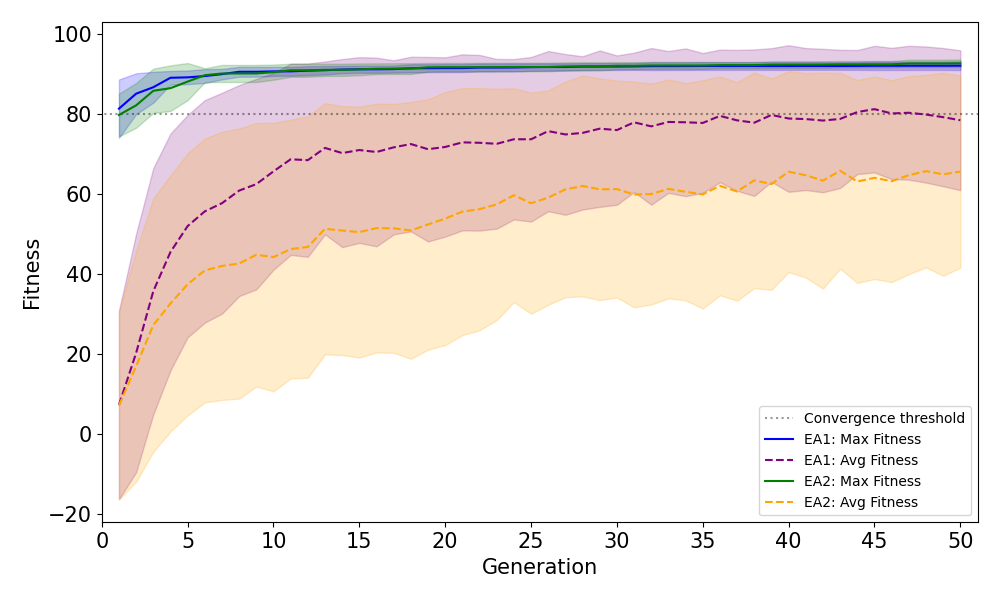
\includegraphics[width=\linewidth]{../../plots/enemy7}
    \caption{}
    \label{fig:enemy7}
\end{figure}
\begin{figure}[htbp]
    \centering
    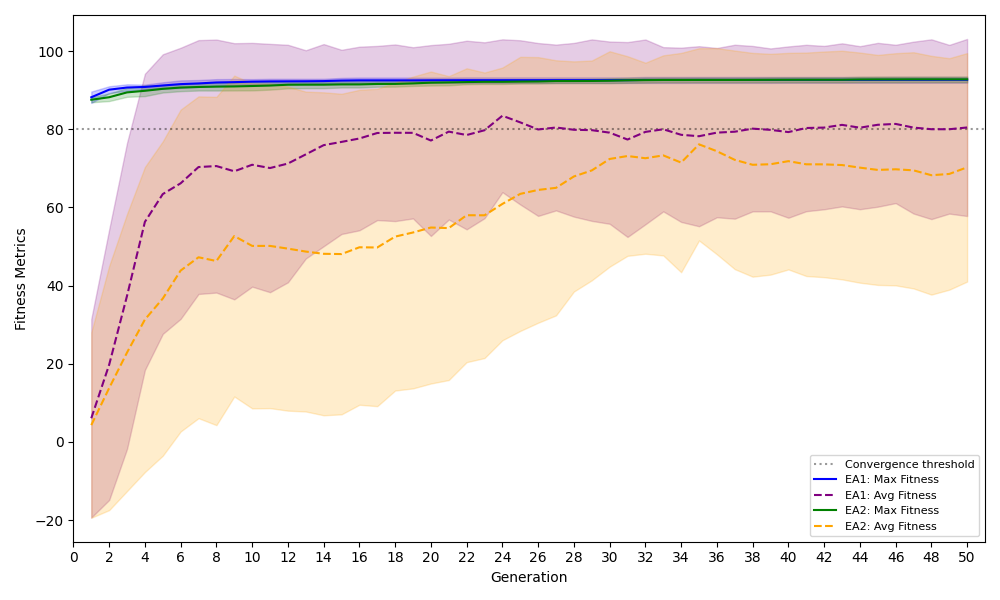
\includegraphics[width=\linewidth]{../../plots/enemy8}
    \caption{}
    \label{fig:enemy8}
\end{figure}

\subsection{Hypothesis 2}
The performance of specialist agents using the Blend Crossover and Two-Point Crossover was assessed across three different enemies.
Table X summarizes the maximum fitness values achieved by each EA.
The results indicate that for Enemy 2 and 8, EA2 (Blend) achieved higher maximum fitness values than EA1 (2Point), even if they were relatively similar.
In contrast, for Enemy 8, EA1 showed higher maximum fitness values.
Considering the SDs of the Maximum Fitness values, Enemy 7 exhibited larger SDs for both EAs.

To get more insides on the results of enemy 7, not aligning with our hypothesis, individual gains using boxplots were examined.
Given that the sample size (N = 5) limits the ability to statistically significance, the boxplot can only be considered as tendencies.
The interquartile ranges of enemy 7 reveal that 50\% of the data for both EAs fall in the same range and the means of are close to each other.
Taking the median into consideration, it can be that the data in EA2 (Blend) is more evenly distributed around the median.
In contrast, EA1 (2point) shows a concentration of values around the median, but with two outliers that influence the IQR and the whisker.
Notably, the median for EA1 is high, whereas the median for EA2 is even negative.

\begin{table}[tbp]
    \begin{tabular}{|l|l|l|}
    \hline
    Enemy              & Crossover method & Maximum fitness \\ \hline
    \multirow{2}{*}{2} & 2-PX             & 94.14           \\ \cline{2-3}
                       & BlendX           & 94.74           \\ \hline
    \multirow{2}{*}{7} & 2-PX             & 94.64           \\ \cline{2-3}
                       & BlendX           & 94.18           \\ \hline
    \multirow{2}{*}{8} & 2-PX             & 93.71           \\ \cline{2-3}
                       & BlendX           & 93.94           \\ \hline
    \end{tabular}
\caption{Maximum achievied fitness values for each enemy and crossover method.}
\end{table}

\section{Discussion}
Comparing the results for both EAs, we can conclude the following.
The Two-Point Crossover operator showed a faster convergence, especially against enemies like Enemy 2, as hypothesized and which is in line with the general advantage of k-point crossovers discussed by Singh and Gupta[CITE].
They also mention that Two-Point crossovers tend to exploit known good solutions by focusing on combining useful schemata, as well as having a tendency of getting trapped in local optima.

On the other hand, the Blend Crossover operator showed more variability and a slower convergence, resulting in greater exploration and avoiding early stagnation.
This aligns with the findings from Singh and Gupta[CITE], who describe the method of the crossover operator as “creates offspring by allowing genes to vary more” (BLX-α) in order to avoid premature convergence and once again demonstrating a higher exploration due to its larger standard deviation across all enemies.

The results for the specialist agent performance showed that for Enemy 2, agents evolved using Two-Point Crossover achieved higher fitness scores earlier.
However, for the more complex enemies, such as Enemies 7 and 8, agents evolved with Blend Crossover showed comparable or improved performance.
Box plots of individual gain indicate that Two-Point Crossover led to higher peaks in fitness against simpler enemies, while Blend Crossover exhibited a more balanced performance across complex scenarios, with more consistent median gains.


%\section{Conclusions}

% possibly Acknowledgments or Appendices
